\documentclass[11pt,openany]{article}

\usepackage{mathtools, commath}
% Packages for formatting
\usepackage[margin=1in]{geometry}
\usepackage{fancyhdr}
\usepackage{enumerate}
\usepackage{graphicx}
\usepackage{kotex}
\usepackage{arydshln} % Include this package
\usepackage{bbding}
\usepackage{amsmath}
\usepackage{amsthm}
\usepackage[dvipsnames,table]{xcolor}
\usepackage{amssymb, amsfonts}
\usepackage{wasysym}
\usepackage{footnote}
\usepackage{tablefootnote}
\usepackage{arydshln} % Include this package

% Fonts
\usepackage[T1]{fontenc}
\usepackage[utf8]{inputenc}
\usepackage{newpxtext,newpxmath}
\usepackage{sectsty}

% Define colors
\definecolor{TealBlue1}{HTML}{0077c2}
\definecolor{TealBlue2}{HTML}{00a5e6}
\definecolor{TealBlue3}{HTML}{b3e0ff}
\definecolor{TealBlue4}{HTML}{00293c}
\definecolor{TealBlue5}{HTML}{e6f7ff}

\definecolor{thmcolor}{RGB}{231, 76, 60}
\definecolor{defcolor}{RGB}{52, 152, 219}
\definecolor{lemcolor}{RGB}{155, 89, 182}
\definecolor{corcolor}{RGB}{46, 204, 113}
\definecolor{procolor}{RGB}{241, 196, 15}

\usepackage{color,soul}
\usepackage{soul}
\newcommand{\mathcolorbox}[2]{\colorbox{#1}{$\displaystyle #2$}}
\usepackage{cancel}
\newcommand\crossout[3][black]{\renewcommand\CancelColor{\color{#1}}\cancelto{#2}{#3}}
\newcommand\ncrossout[2][black]{\renewcommand\CancelColor{\color{#1}}\cancel{#2}}

\usepackage{hyperref}
\usepackage{booktabs}

% Chapter formatting
\definecolor{titleTealBlue}{RGB}{0,53,128}
\usepackage{titlesec}
\titleformat{\section}
{\normalfont\sffamily\Large\bfseries\color{titleTealBlue!100!gray}}{\thesection}{1em}{}
\titleformat{\subsection}
{\normalfont\sffamily\large\bfseries\color{titleTealBlue!50!gray}}{\thesubsection}{1em}{}

%Tcolorbox
\usepackage[most]{tcolorbox}
\usepackage{multirow}
\usepackage{multicol}
\usepackage{blindtext}

\usepackage[linesnumbered,ruled]{algorithm2e}
\usepackage{algpseudocode}
\usepackage{setspace}
\SetKwComment{Comment}{/* }{ */}
\SetKwProg{Fn}{Function}{:}{end}
\SetKw{End}{end}
\SetKw{DownTo}{downto}

% Define a new environment for algorithms without line numbers
\newenvironment{algorithm2}[1][]{
	% Save the current state of the algorithm counter
	\newcounter{tempCounter}
	\setcounter{tempCounter}{\value{algocf}}
	% redefine the algorithm numbering (remove prefix)
	\renewcommand{\thealgocf}{}
	\begin{algorithm}
	}{
	\end{algorithm}
	% Restore the algorithm counter state
	\setcounter{algocf}{\value{tempCounter}}
}

\usepackage{adjustbox}
% Header and footer formatting
\pagestyle{fancy}
\fancyhead{}
\fancyhf{}
\rhead{\textcolor{TealBlue2}{\large\textbf{리만의 복소해석을 토대로 얻는 내 수학적 시야 (2기)}}}%\rule{3cm}{0.4pt}}
\lhead{\textcolor{TealBlue2}{\large\textbf{수학의 즐거움, Enjoying Math}}}
% Define footer
%\newcommand{\footer}[1]{
%\begin{flushright}
%	\vspace{2em}
%	\includegraphics[width=2.5cm]{school_logo.jpg} \\
%	\vspace{1em}
%	\textcolor{TealBlue2}{\small\textbf{#1}}
%\end{flushright}
%}
%\rfoot{\large Department of Information Security, Cryptogrphy and Mathematics, Kookmin Uni.\includegraphics[height=1.5cm]{school_logo.jpg}}
\fancyfoot{}
\fancyfoot[C]{-\thepage-}

\usepackage{tcolorbox}
\tcbset{colback=white, arc=5pt}

\definecolor{axiomcolor}{HTML}{a88bfa}
\definecolor{defcolor}{RGB}{52, 152, 219}
\definecolor{procolor}{RGB}{241, 196, 15}
\definecolor{thmcolor}{RGB}{231, 76, 60}
\definecolor{lemcolor}{RGB}{155, 89, 182}
\definecolor{corcolor}{RGB}{46, 204, 113}
\definecolor{execolor}{RGB}{90, 128, 127}

% Define a new command for the custom tcolorbox
\newcommand{\axiombox}[2][]{%
	\begin{tcolorbox}[colframe=axiomcolor, title={\color{white}\bfseries #1}]
		#2
	\end{tcolorbox}
}

\newcommand{\defbox}[2][]{%
	\begin{tcolorbox}[colframe=defcolor, title={\color{white}\bfseries #1}]
		#2
	\end{tcolorbox}
}

\newcommand{\lembox}[2][]{%
	\begin{tcolorbox}[colframe=lemcolor, title={\color{white}\bfseries #1}]
		#2
	\end{tcolorbox}
}

\newcommand{\probox}[2][]{%
	\begin{tcolorbox}[colframe=procolor, title={\color{white}\bfseries #1}]
		#2
	\end{tcolorbox}
}

\newcommand{\thmbox}[2][]{%
	\begin{tcolorbox}[colframe=thmcolor, title={\color{white}\bfseries #1}]
		#2
	\end{tcolorbox}
}

\newcommand{\corbox}[2][]{%
	\begin{tcolorbox}[colframe=corcolor, title={\color{white}\bfseries #1}]
		#2
	\end{tcolorbox}
}



\usepackage{amsthm}

% Define custom theorem styles
\newtheoremstyle{dotless} % Name of the style
{3pt} % Space above
{3pt} % Space below
{\itshape} % Body font
{} % Indent amount
{\bfseries} % Theorem head font
{} % Punctuation after theorem head
{2.5mm} % Space after theorem head
{} % Theorem head spec

\newtheoremstyle{definitionstyle} % Name of the style
{3pt} % Space above
{3pt} % Space below
{} % Body font
{} % Indent amount
{\bfseries} % Theorem head font
{.} % Punctuation after theorem head
{2.5mm} % Space after theorem head
{} % Theorem head spec

% Applying custom styles
\theoremstyle{dotless}
\newtheorem{theorem}{Theorem} % Theorem environment with section-wise numbering
\newtheorem{proposition}[theorem]{Proposition} % Theorem environment with section-wise numbering
\newtheorem{lemma}[theorem]{Lemma} % Lemma shares the counter with theorem
\newtheorem{corollary}[theorem]{Corollary} % Corollary shares the counter with theorem

\theoremstyle{definitionstyle}
\newtheorem*{observation}{\textcolor{Magenta}{Observation}}
\newtheorem{definition}{Definition} % Definition shares the counter with theorem
\newtheorem{example}{Example} % Example shares the counter with theorem
\newtheorem{exercise}{Exercise} % Example shares the counter with theorem
\newtheorem{remark}{Remark} % Remark shares the counter with theorem
\newtheorem*{note}{Note}

\newtheorem*{definition*}{Definition} % Definition shares the counter with theorem
\newtheorem*{example*}{Example} % Example shares the counter with theorem
\newtheorem*{exercise*}{\textcolor{violet}{Exercise}} % Example shares the counter with theorem
\newtheorem*{remark*}{Remark} % Remark shares the counter with theorem


\usepackage{tikz}
\usepackage{tikz-cd}
\usepackage{tikz-3dplot}
\usepackage{pgfplots}
\pgfplotsset{compat=newest} % Adjust to your version of pgfplots
\def\Circlearrowleft{\ensuremath{%
		\rotatebox[origin=c]{180}{$\circlearrowleft$}}}
\def\Circlearrowright{\ensuremath{%
		\rotatebox[origin=c]{180}{$\circlearrowright$}}}
\def\CircleArrowleft{\ensuremath{%
		\reflectbox{\rotatebox[origin=c]{180}{$\circlearrowleft$}}}}
\def\CircleArrowright{\ensuremath{%
		\reflectbox{\rotatebox[origin=c]{180}{$\circlearrowright$}}}}
\usetikzlibrary{
	3d, % For 3D drawing
	angles,
	arrows,
	arrows.meta,
	backgrounds,
	bending,
	calc,
	decorations.pathmorphing,
	decorations.pathreplacing,
	decorations.markings,
	fit,
	matrix,
	patterns,
	patterns.meta,
	positioning,
	quotes,
	shadows,
	shapes,
	shapes.geometric,
	tikzmark
}
\tikzset{
	% single mid‐path arrow
	mid arrow/.style={
		decoration={
			markings,
			mark=at position 0.5 with {\arrow{Stealth[scale=1.2]}}
		},
		postaction={decorate},
	},
	% style for field arrows
	field arrow/.style={
		-{Stealth[scale=1.0]},
		thick,
		blue!70!black,
	},
}
\newcommand{\ie}{\textnormal{i.e.}}
\newcommand{\rsa}{\mathsf{RSA}}
\newcommand{\rsacrt}{\mathsf{RSA}\textendash\mathsf{CRT}}
\newcommand{\inv}[1]{#1^{-1}}

%New Command
%\newcommand{\set}[1]{\left\{#1\right\}}
\newcommand{\N}{\mathbb{N}}
\newcommand{\Z}{\mathbb{Z}}
\newcommand{\Q}{\mathbb{Q}}
\newcommand{\R}{\mathbb{R}}
\newcommand{\cR}{\mathcal{R}}
\newcommand{\C}{\mathbb{C}}
\newcommand{\F}{\mathbb{F}}
\newcommand{\nbhd}{\mathcal{N}}
\newcommand{\Log}{\operatorname{Log}}
\newcommand{\Arg}{\operatorname{Arg}}
\newcommand{\pv}{\operatorname{P.V.}}

\newcommand{\of}[1]{\left( #1 \right)} 
%\newcommand{\abs}[1]{\left\lvert #1 \right\rvert}
%\newcommand{\norm}[1]{\left\| #1 \right\|}

\newcommand{\sol}{\textcolor{magenta}{\bf Sol}}
\newcommand{\conjugate}[1]{\overline{#1}}

\newcommand{\res}{\operatorname{res}}
\DeclareMathOperator*{\Res}{\operatorname{Res}}

%\renewcommand{\Re}{\operatorname{Re}}
%\renewcommand{\Im}{\operatorname{Im}}

\newcommand{\cyclic}[1]{\langle #1 \rangle}
\newcommand{\uniform}{\overset{\$}{\leftarrow}}
\newcommand{\xmark}{\textcolor{red}{\XSolidBrush}}
\newcommand{\vmark}{\textcolor{green!75!black}{\CheckmarkBold}}

\newcommand{\gen}[1]{\langle #1 \rangle}
\newcommand{\Gen}[1]{\left\langle #1 \right\rangle}

\newcommand{\img}[1]{\text{Img}(#1)}
\newcommand{\Img}[1]{\text{Img}\left(#1\right)}
\newcommand{\preimg}[1]{\text{Img}^{-1}(#1)}
\newcommand{\Preimg}[1]{\text{Img}^{-1}\left(#1\right)}

\newcommand{\relation}{\mathrel{\mathcal{R}}}
\newcommand{\injection}{\rightarrowtail}
\newcommand{\surjection}{\twoheadrightarrow}
\newcommand{\id}{\textnormal{id}}

\newcommand{\eqclass}[1]{\left[#1\right]}

% Define custom colors for O and X
\newcommand{\yes}{\textcolor{blue}{\bf \fullmoon}}
\newcommand{\no}{\textcolor{red}{\bf \texttimes}}

\DeclarePairedDelimiter\ceil{\lceil}{\rceil}
\DeclarePairedDelimiter\floor{\lfloor}{\rfloor}
%\renewcommand{\floor}[#1]{\lfloor #1\rfloor}
%\newcommand{\Floor}[#1]{\left\lfloor #1\right\rfloor}
%\newcommand{\ceil}[#1]{\lceil #1\rceil}
%\newcommand{\Ceil}[#1]{\left\lceil #1\right\rceil}

\newcommand{\topology}{\mathscr{T}}
\newcommand{\sequence}[1]{\langle #1\rangle}

% Topology
%\newcommand{\nbhd}{\mathcal{N}}

% Linear Algebra
\newcommand{\Span}{\operatorname{\normalfont span}}
\newcommand{\basis}{\mathcal{B}}
\newcommand{\card}[1]{\text{\normalfont card}(#1)}
\renewcommand{\vec}[1]{\mathbf{#1}}
\setstretch{1.25}

%\usepackage{background}
%\backgroundsetup{
%	scale=3,
%	color=gray!20,
%	opacity=0.3,
%	angle=45,
%	contents={\Huge \sffamily Ji, Yong-hyeon}
%}
\begin{document}
\pagenumbering{arabic}
\begin{center}
	\huge\textbf{Line Integral I}\\
	\vspace{0.5em}
	\large{Ji, Yong-hyeon}\\
%	\large{\ttfamily \url{https://github.com/Hacker-Code-J}}\\
	\vspace{0.5em}
	\normalsize{\today}\\
\end{center}

\noindent 
We cover the following topics in this note.
\begin{itemize}
	\item TBA.
\end{itemize}
\hrule\vspace{12pt}
%\tableofcontents
%\newpage

\section*{Preliminaries}
Let \( I = [a,b] \subset \mathbb{R} \) and let 
\[
\gamma : I \to \mathbb{R}^n
\]
be a piecewise \( C^1 \) mapping whose image \( \gamma(I) \) is the curve along which integration is performed. For any partition 
\[
\mathcal{P} = \{t_0, t_1, \ldots, t_N\} \quad \text{with} \quad a = t_0 < t_1 < \cdots < t_N = b,
\]
define the mesh of the partition by
\[
\|\mathcal{P}\| := \max_{1 \le i \le N} (t_i - t_{i-1}).
\]
For each subinterval \([t_{i-1}, t_i]\), choose a sample point \(\xi_i \in [t_{i-1}, t_i]\).

\section*{Line Integral of a Scalar Function}
Let 
\[
f : \gamma(I) \to \mathbb{R}
\]
be a continuous function. Define the Riemann sum by
\[
S(\mathcal{P}, \{\xi_i\}) := \sum_{i=1}^N f\bigl(\gamma(\xi_i)\bigr) \, \|\gamma(t_i)-\gamma(t_{i-1})\|.
\]
Then the \emph{line integral of \(f\) along \(\gamma\) with respect to arc length} is defined by
\[
\int_{\gamma} f \, ds := \lim_{\|\mathcal{P}\| \to 0} S(\mathcal{P}, \{\xi_i\}),
\]
provided that the limit exists and is independent of the choice of partition \(\mathcal{P}\) and sample points \(\{\xi_i\}\).

In the case that \(\gamma\) is continuously differentiable, the definition is equivalent to
\[
\int_{\gamma} f \, ds = \int_a^b f\bigl(\gamma(t)\bigr) \, \|\gamma'(t)\|\,dt.
\]

\section*{Line Integral of a Vector Field}
Let 
\[
\mathbf{F} : \gamma(I) \to \mathbb{R}^n
\]
be a continuous vector field. Using the same partition \(\mathcal{P}\) and sample points \(\{\xi_i\}\) as above, define the Riemann sum
\[
S(\mathcal{P}, \{\xi_i\}) := \sum_{i=1}^N \mathbf{F}\bigl(\gamma(\xi_i)\bigr) \cdot \bigl(\gamma(t_i)-\gamma(t_{i-1})\bigr),
\]
where ``\(\cdot\)'' denotes the standard Euclidean dot product. The \emph{line integral of \(\mathbf{F}\) along \(\gamma\)} is then defined by
\[
\int_{\gamma} \mathbf{F} \cdot d\mathbf{r} := \lim_{\|\mathcal{P}\| \to 0} S(\mathcal{P}, \{\xi_i\}),
\]
provided that the limit exists independently of the partition and the choice of sample points.

If \(\gamma\) is continuously differentiable, this definition is equivalent to
\[
\int_{\gamma} \mathbf{F} \cdot d\mathbf{r} = \int_a^b \mathbf{F}\bigl(\gamma(t)\bigr) \cdot \gamma'(t)\,dt.
\]

\newpage
Formal Definition (Scalar Line Integral):

Let 
\[
\gamma : [a,b] \longrightarrow \mathbb{R}^n
\]
be a piecewise continuously differentiable (and hence rectifiable) parameterization of a curve \( C \subset \mathbb{R}^n \), and let 
\[
f : C \to \mathbb{R}
\]
be a continuous function. Denote by \(\|\gamma'(t)\|\) the norm of the derivative of \(\gamma\) at \(t\). Then the *line integral* (or *integral of \(f\) with respect to arc length*) is defined by

\[
\int_C f\, ds \; := \; \lim_{\|\Delta\|\to 0} \sum_{i=1}^{N} f\Bigl(\gamma(t_i^*)\Bigr)\,\Bigl\|\gamma(t_i)-\gamma(t_{i-1})\Bigr\|,
\]
where \(\{t_0, t_1, \dots, t_N\}\) is an arbitrary partition of \([a,b]\) with mesh \(\|\Delta\| = \max_{1 \le i \le N}(t_i-t_{i-1})\) and \(t_i^* \in [t_{i-1}, t_i]\). Under the hypothesis that \(\gamma\) is continuously differentiable, one may equivalently express the line integral as
\[
\int_C f\, ds \; = \; \int_a^b f\bigl(\gamma(t)\bigr)\,\|\gamma'(t)\|\,dt.
\]

A similar construction yields the definition of the line integral of a vector field \(\mathbf{F} : U \subset \mathbb{R}^n \to \mathbb{R}^n\) along \(C\):
\[
\int_C \mathbf{F} \cdot d\mathbf{s} \; := \; \int_a^b \mathbf{F}\bigl(\gamma(t)\bigr) \cdot \gamma'(t)\,dt.
\]

	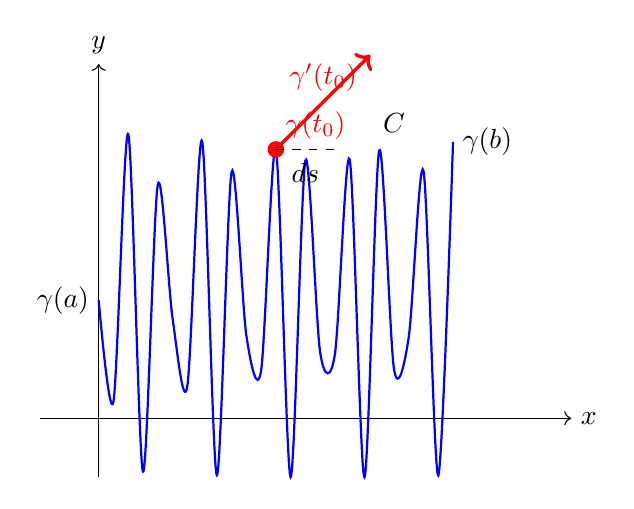
\begin{tikzpicture}[scale=1.5]
		% Axes
		\draw[->] (-0.5,0) -- (4,0) node[right] {$x$};
		\draw[->] (0,-0.5) -- (0,3) node[above] {$y$};
		
		% Parameterized curve gamma: example curve in R^2
		\draw[thick, blue, domain=0:3, smooth, variable=\t] 
		plot ({\t}, {1.5*sin(30*\t r) + 1});
		\node at (2.5,2.5) {$C$};
		
		% Endpoints of the curve
		\node at (0, {1.5*sin(0 r)+1}) [left] {$\gamma(a)$};
		\node at (3, {1.5*sin(90 r)+1}) [right] {$\gamma(b)$};
		
		% Mark a sample point gamma(t_0)
		\pgfmathsetmacro{\tzero}{1.5}
		\pgfmathsetmacro{\x}{\tzero}
		\pgfmathsetmacro{\y}{1.5*sin(30*\tzero r)+1}
		\fill[red] (\x, \y) circle (2pt) node[above right] {$\gamma(t_0)$};
		
		% Draw tangent vector at gamma(t_0)
		% (Here the vector is chosen illustratively.)
		\pgfmathsetmacro{\dx}{0.8}
		\pgfmathsetmacro{\dy}{0.8}
		\draw[->, very thick, red] (\x, \y) -- ++({\dx}, {\dy}) node[midway, above] {$\gamma'(t_0)$};
		
		% Indicate differential arc-length element ds
		\draw[dashed] (\x, \y) -- ++({0.5}, {0});
		\node at (\x+0.25, \y-0.2) {$ds$};
	\end{tikzpicture}
\vfill
\begin{thebibliography}{9}
	\bibitem{riemann_0}
	수학의 즐거움, Enjoying Math. ``[리만의 복소해석을 토대로 얻는 내 수학적 시야] 0. 오리엔테이션'' YouTube Video, 1:49:27. Published 
	September 4, 2023. URL: \url{https://www.youtube.com/watch?v=EovxcF_DG_k&list=PL4m4z_pFWq2ob-P9m3SQZPyHTaJbbkvdz}.
	\bibitem{riemann_1}
	수학의 즐거움, Enjoying Math. ``[리만의 복소해석을 토대로 얻는 내 수학적 시야] 1. 선적분의 정의에 대한 디스커션'' YouTube Video, 1:58:19. Published 
	September 11, 2023. URL: \url{https://www.youtube.com/watch?v=zoalSFi1RKo&list=PL4m4z_pFWq2ob-P9m3SQZPyHTaJbbkvdz&index=2}.
\end{thebibliography}

%\newpage
%\appendix
%\section{Proof of Zorn's Lemma from Axiom of Choice}
%\thmbox{\begin{theorem*}\hypertarget{zorn}{}
%The following statements are equivalent: \begin{enumerate}
%	\item \textbf{Axiom of Choice (AC)}:\quad For every indexed family $\set{S_i}_{i\in I}$ of nonempty sets, there exists a choice function $f:I\to\bigcup_{i\in I}S_i$ such that $f(i)\in X_i$ for all $i\in I$.
%	\item \textbf{Zorn's Lemma}:\quad If $(P,\preceq)$ is a nonempty partially ordered set in which every chains has an upper bound in $P$, then $P$ contains at least one maximal element.
%\end{enumerate}
%\end{theorem*}}
%\begin{proof}
%\begin{itemize}
%	\item[($\Rightarrow$)] $(\textbf{AC}\implies \textbf{ZL})$ Assume that the Axiom of Choice holds.
%	\begin{enumerate}
%		\item \textbf{Definition of Poset}
%		
%		Let $(P,\preceq)$ be a nonempty partially ordered set with the property that every chain in $P$ has an upper bound in  $P$.
%		
%		\item \textbf{Construction of an Extending Function}
%		
%		Define the family $\set{\mathcal{C}_i}_{i\in I}$ of chains in $P$. For any chain $\mathcal{C}_i$ that is not maximal with respect to inclusion (\ie, $\exists $), AC guarantees that we can elect an element \[
%		f(C)
%		\] 
%	\end{enumerate}
%	\item[($\Leftarrow$)] $(\textbf{ZL}\implies \textbf{AC})$ 
%\end{itemize}
%\end{proof}
\end{document}
